\section{Алгебра логических значений}
Алгебра Буля $B = (\{0, 1\}, \lor, \land, ')$ полезна, когда необходимо применить в логике математические методы.

Операция $x \lor y$ также обозначается как $x \cup y$ или $x + y$.

Операция $x \land y$ также обозначается как $x \cap y$ или $x \cdot y$.

\subsection{Булевы многочлены и булевы функции}
\dftion \textbf{Булевы многочлены} --- формулы, образованные ил булевых переменных $x, y, \dots$ и симвлов булквых операций $', +, \cdot$ по следующим правилам:
\begin{enumerate}
    \item Все булевы переменные и символы 0, 1 являются булевыми многочленами
    \item Если $p$ и $q$ --- булевы многочлены, то $p'$, $p+q$, $pq$ --- тоже многочлены
\end{enumerate}
Множество всех булевых многочленов обозначается $P_n$.

\dftion Каждый булев многочлен $p(x_1, \dots, x_n)$ определяет отображение $\vec p : B^n \to B$, которое называется \textbf{булевой полиномиальной функией}. Булевы многочлены называются \textit{эквивалентными}, если определяют одну и ту же булеву полиномиальную функцию.
\subsection{Системы булевых функций}
\dftion \textbf{Суперпозция} булевых функций $g(y_1, \dots, y_m)$ и $f_1(x_1, \dots, x_n)$, \dots, $f_m(x_1, \dots, x_n)$ --- булева функция $f(x_1, \dots, x_n)$, значения которой определяются по формуле:
$$f(x_1, \dots, x_n) = g(h_1(x_1, \dots, x_n), \dots, h_m(x_1, \dots, x_n))$$

Для упрощения записи суперпозиции булевых функций скобки по возможности опускаются с учётом следующего приоритета булевых функций: $', \cdot$ и затем все остальные булевы функции.

\dftion Система булевых функций $F = \{f_1, \dots, f_n\}$ называется \textbf{полной}, если любая функция может быть представлена в виде суперпозиции из этой системы $F$.
\subsection{Классы и теорема Поста}
\dftion \textbf{Классы Поста} --- $L$, $S$, $M$, $P_0$, $P_1$ --- линейные, самодвойственные, монотонные... функции.
\dftion \textbf{Теорема Жегалкина}. Любая функция $f$ может быть представлена в виде полинома Жегалкина
$$f(x_1, \dots, x_n) = \underset{j_1, \dots, j_k} \oplus x_{i_1}x_{i_k} \oplus c$$
для некоторых значений $c \in \{0,1\}$ и $1 < i_1 < \dots < i_k \leq n$. Причём такое разложение единственно с точностью до порядка слагаемых.

\dftion \textbf{Линейная} булева функция --- функция, многочлен Жегалкина которой не содержит произведения переменных.

\dftion \textbf{Самодостаточная} булева функция выполняет условие $f(x_1,$ $\dots,$ $x_n) =$ $(f(x_1', \dots, x_n'))'$.

\dftion \textbf{Монотонная} булева функция выполняет условие

$\forall x_1, y_1, \dots, x_n, y_n \in B \; x_1 \leq y_1, \dots, x_n \leq y_n \then f(x_1, \dots, x_n) \leq f(y_1, \dots, y_n)$

\dftion $P_0$ --- класс всех булевых функций, удовлетворяющих условию $f(0,\dots,0)=0$.

\dftion $P_1$ --- класс всех булевых функций, удовлетворяющих условию $f(1,\dots,1)=1$.

\dftion \textbf{Теорема Поста}. Система фнукций является \textbf{полной} тогда и только тогда, когда она не содержится ни в одном из классов Поста.

\underline{Алгоритм доказательства системы булевых функций} $F = \{f_1, \dots, f_n\}$:
\begin{enumerate}
    \item Строим таблицу, в которой столбцы соответствуют классам Поста $L, S, M, P_0, P_1$, а строки --- функциям $f_1, \dots, f_k$
    \item Для каждой функции на пересечениях со столбцами помечаем, соответствует ли она данному классу Поста
    \item Система функций является полной, если ни одна функция не оказалась принадлежащей какому бы то ни было классу Поста
\end{enumerate}
\subsection{Переключательные схемы}
Рассматриваются электрические ПС, представляющие собой соединённые проводниками переключатели и источники тока.

Условимся обозначать символом 1 протекание тока в проводниках и символом 0 --- отсутствие тока в проводниках.

\dftion \textbf{Переключатель} --- электромагнитное реле с контактами и индукционной катушкой, состояние которой медлируется булевой переменной $x$: $x = 1$ --- в катушке идёт ток, и $x = 0$ --- в катушке тока нет.

Контакты реле --- замыкающие или размыкающие.

Через \textit{замыкающий контакт} реле ток проходит в том и только в том случае, если $x = 1$ --- такой контакт моделируется булевой переменной $x$.

Через \textit{размыкающий контакт} реле ток проходит в том и только в том случае, если $x = 0$ --- такой контакт моделируется отрицанием булевой переменной $x'$.

Переключатели $p, q$ могут быть соединены последовательно и параллельно. Через последовательно соединённые переключатели ток проходит в том и только в том случае, если $p=q=1$ --- такое соединение моделируется булевым многочленом $pq$.

Через параллельно соединённые переключатели $p,q$ ток не проходит в том и только в том случае, если $p=q=0$ --- такое соединение моделируется булевым многочленом $p+q$.

В результате любая электрическая ПС моделируется некоторым булевым многочленом $p$, который принимает значение 1 в том и только в том случае, если в ПС идёт ток.

Соответствующая такому многочлену $p$ булева функция $p$ называется \textit{функцией проводимости} ПС, так как она показывает, при каких значениях булевых переменных (т. е. переключателей данной схемы) в ПС идёт электрический ток.

Преключательную схему с функцией проводимости $p=p(x_1,\dots,x_n)$ можно представлять в виде устройства с $n$ входами и одним выходом, которое преобразует входные булевы значения $x_1 = \alpha_1, \dots, x_n = \alpha_n$ в выходное булево значение $\vec p(\alpha_1, \dots, \alpha_n)$.

Простейшие булевы многочлены моделируют ПС, которые называются \textit{логическими элементами} (или \textit{вентилями}) и обозначаются специальными диаграммами.

\begin{tabular}{ccc}
    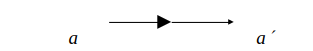
\includegraphics[scale=0.35]{графика/not.png} & \includegraphics[scale=0.35]{графика/and.png} & 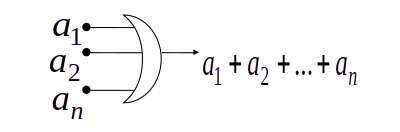
\includegraphics[scale=0.35]{графика/or.png} \\
    NOT-элемент & AND-элемент & OR-элемент
\end{tabular}
\subsection{Минимизация булевых многочленов}
Рассмотрим вопрос минимизации ДНФ $p$. Конъюнкт $q$ называется \textit{импликантом} формы $p$, если $pq = q$. Импликанты, минимальные по числу вхождений в них булевых переменных, называются $\textit{простыми импликантами}$. Дизъюнкция всех простых импликант формы $p$ называется $\textit{сокращённой ДНФ}$.

\textbf{Лемма 1}. Любая ДНФ $p$ эквивалентна некоторой сокращённой ДНФ.

Совершненную ДНФ формы $p$ можно получить $\textit{методом Квайна}$ с помощью последовательного применения следующих двух видов сокращений:
\begin{enumerate}
    \item \textit{операция склеивания}, которая для конъюнктов $q$ и булевых переменных $x$ определяется по формуле: $$qx + qx' = qx + qx' + q$$
    \item \textit{операция поглощения}, которая для конъюнктов $q$, булевых переменных $x$ и значений $\alpha \in \{0, 1\}$ определяется по формуле: $$qx^\alpha + q = q.$$
\end{enumerate}

\underline{Лемма 2}. Любая ДНФ $p$ эквивалентна некоторой минимальной ДНФ.

Минимальная ДНФ формы $p$ получается с помощью \textit{матрицы Квайна}:
\begin{itemize}
    \item столбцы матрицы помечаются конъюнктами $p_1, \dots, p_m$ формы $p$;
    \item строки матрицы помечаются импликантами $q_1,\dots,q_k$ сокращённой ДНФ формы $p$
    \item на пересечении строки $q_i$ и столбца $p_j$ ставится символ *, если импликант $q_i$ является частью конъюнкта $p_j$.
\end{itemize}

Тупиковые ДНФ --- дизъюнкции тех минимальных наборов импликант, в которых имеются звёздочки для всех столбцов матрицы Квайна.

Тупиковые ДНФ с наименьшим числом вхождений булевых переменных являются искомыми минимальными ДНФ формы $p$.